% !TEX root = main.tex

\chapter{Motivation}
\label{ch:motivation}
\noindent

\newcommand{\officialp}{official prose}
\newcommand{\spectecp}{SpecTec prose}

\begin{figure}[h!]
    \centerline{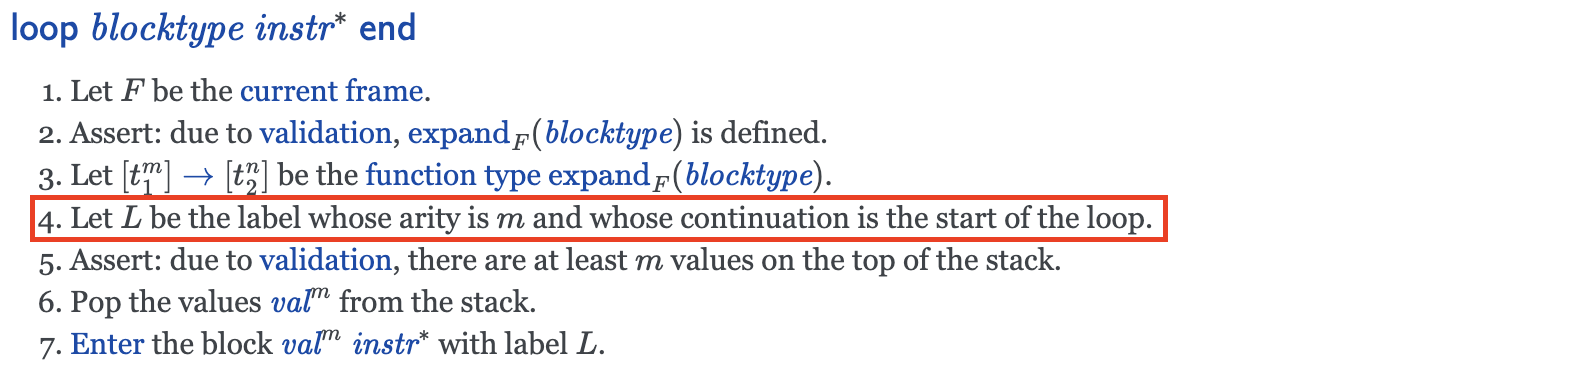
\includegraphics[width=15cm]{fig/loop}}
    \caption[Enter the caption title here]{\texttt{loop} instruction} \label{loop-fig}
    \centerline{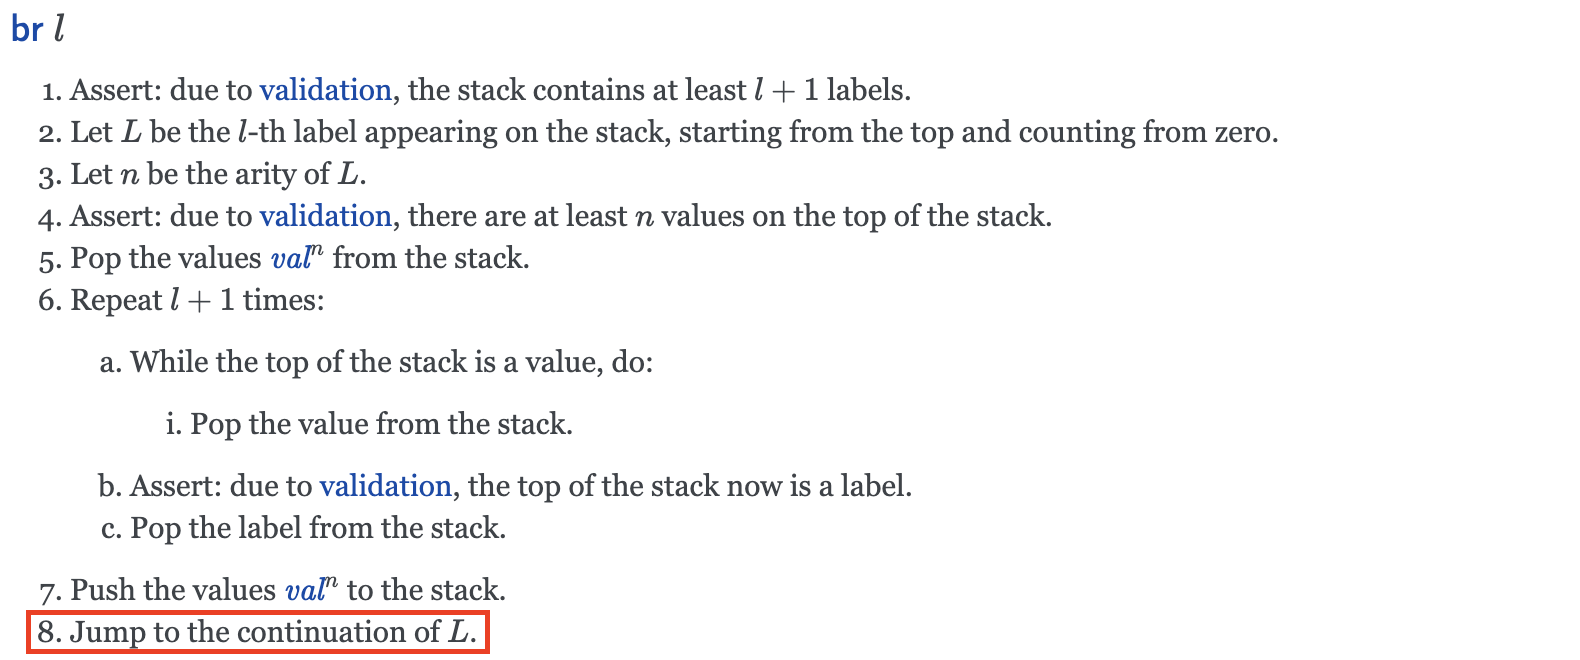
\includegraphics[width=15cm]{fig/br}}
    \caption[Enter the caption title here]{\texttt{br} instruction} \label{br-fig}
\end{figure}
TODO: remove redundant part in the fig

It might be easy to understand how the \officialp{} explains the control flow
of WebAssembly, if we assume that a WebAssembly code is loaded on a memory and
a pc points to the instruction to execute.
To describe control flow, it uses a structure named \textit{block} which
consitutes of a instruction sequence.
When executing the instruction sequence inside the block, it can jump to the
starting point of the block or the end of the block.
For example, \cref{loop-fig} is the \officialp{} \texttt{loop} instruction.
It says that the continuation is the start of the loop and the information is
stored in a label, which is pushed in the stack when
entering the block.
\cref{br-fig} is a \texttt{br} instruction in the \officialp{}.
According to it, if the \texttt{br} instruction in the block is executed to
branch out the block, the label is popped in the stack and jumps to the
continuation of the label, which is the start of the loop instruction.

TODO: detailed explanation of \spectecp{} w/ fig

However, rather than using the notion like pc, the \spectecp{} assumes that the
\red{machine} takes WebAssembly instructions one by one, and changes the
internal state accordingly.
This is because the \spectecp{} is generated automatically from the \red{dsl}
which doesn't model the pc.
As a result, rather than jump to the start of the loop, \spectecp{} stores the
\texttt{loop} instruction in the label, and executes it again if \texttt{br}
instruction is executed.

don't remember end!





% official spec prose notation control structure
% seems to be pc-based
% AL from DSL ~ formal notation: no pc
% AL: instruction sequence input continously
% device exit semantics for AL
% Executable spec passes all wasm testcases
% weird, maybe not happened in realworld, but valid wasm code
% wrong!
